\section{Model Translation}
Model representation in the PRA domain is encumbered by format fragmentation and proprietary development practices. A small group of stakeholders, each using specialized file structures, has little incentive to converge on a single standard. Proposing a new "universal" format can inadvertently add yet another layer of fragmentation if adoption proves limited. Conversely, attempting a fully connected translation map among all existing formats is a significant undertaking, requiring both ongoing maintenance and broad community participation that may not materialize.

\subsection{PRAcciolini: Translation without a Single Intermediate Representation}
In view of these constraints, the short-term strategy is to create a system of lightweight interfaces under an open-source tool, referred to here as \emph{PRAcciolini}, that interlinks existing translation tools without defaulting to a single pivot format. Rather than striving for every possible conversion path, the goal is to form what might be called a "translation spanning tree": a subset of connections that covers most practical needs while avoiding excessive overhead. This design allows each domain-specific library to retain its native parsing and exporting routines, with conversions performed only when required.

\begin{figure}[h!]
  \includesvg[width=\textwidth]{3_identifying_gaps/benchmarking/datasets/translation/figs/translations-pracciolini.svg}
    \caption{Example of supported model translations in PRAcciolini.}
  \label{fig:translations}
\end{figure}

As shown in Figure~\ref{fig:translations}, a CAFTA XML file can be transformed into FTREX FTP or SAPHSOLVE JSON, while MAR-D data can be republished as OpenPSA XML and potentially mapped to a TensorFlow-compatible format. Round-trip testing (translating from one format to another and back again) verifies fidelity, ensuring that essential model information remains intact. By removing the need for a monolithic "canonical" structure, this partial translation network can remain both flexible and modular, minimizing risky lock-step updates whenever new releases or extensions emerge.

\subsection{Long-Term Goal: OpenPRA JSON Schema}
The long-term initiative extends beyond partial connectivity to propose an openly licensed JSON schema (OpenPRA JSON). This plan intends to balance retained compatibility with existing standards (e.g., OpenPSA XML) against the specialized requirements of nuclear licensing. Two major factors underlie this choice:

\begin{itemize}
\item \textbf{Extensibility and Clarity:} JSON natively supports hierarchical key-value pairs that facilitate both human readability and efficient parsing. PRA models tend to store domain-specific knowledge, not merely numeric parameters, making readability a high priority. Unlike FlatBuffers or similar purely binary formats, JSON offers a middle ground by allowing large, descriptive models without sacrificing parser performance.
\item \textbf{Nuclear-Specific Needs:} Although OpenPSA XML has served as a standard in probabilistic safety, it is no longer actively maintained. The OpenPRA JSON schema seeks to preserve core OpenPSA semantics while adding a namespace dedicated to nuclear regulation. This extension accommodates plant-specific elements and licensing-related fields that exceed the scope of general probabilistic models.
\end{itemize}

Thus, the near-term effort builds a manageable translation spanning tree through PRAcciolini, minimizing integration burdens across multiple closed-source tools. Simultaneously, OpenPRA JSON emerges as a robust, future-facing schema for those organizations requiring more comprehensive and domain-tailored data structures. This dual approach, maintaining workable interoperability while evolving a modern open standard, addresses both the immediate priorities of the PRA community and the long-term need for a sustainable, extensible foundation.

% A persistent challenge in PRA software development is the variety and fragmentation of data formats. In a domain with comparatively few stakeholders, introducing yet another universal format frequently aggravates fragmentation rather than alleviating it. At the same time, providing full interoperability among all existing formats is likewise complex, given both the number of competing syntaxes and limited incentives in predominantly closed development communities.

% In response, we are implementing an open framework that focuses on systematic translation rather than any single, newly imposed format. Central to this strategy is a flexible open-source schema, OpenPRA JSON, designed to accommodate content from external formats wherever possible. Since OpenPSA XML is widely recognized as the de facto industry standard, our immediate emphasis lies in translating to and from OpenPSA XML. However, we do not require model data to adhere strictly to the OpenPRA JSON layout; each grammar or file type can continue to use its own native parsing and serialization.

% As shown in Figure~\ref{fig:translations}, this setup allows direct "bridges" among formats. Tools like FTREX FTP or SAPHIRE JSON remain parsed by their existing libraries, then converted into others on demand without mandating a monolithic pivot. For instance, a MAR-D representation can be validated by its native routines and output as OpenPSA XML or even transformed into TensorFlow Graph form. Likewise, CAFTA XML may flow directly into FTREX FTP or SAPHSOLVE JSON. Overall, the architecture constructs a mesh of translators leveraging format-specific toolkits yet avoids imposing a unitary, intermediate data structure.

% A major complicating factor in tool development in the PRA domain is model representation and exchange. As a direct consequence of closed-sourced development practices, format/syntax fragmentation is a non-trivial problem. At the same time, the number of stakeholders in the PRA field is also quite limited. All this to say, for such a niche and already fragmented field, creating a *new* format (with the purehearted intent of unifying all others) actually tends to have the opposite effect.

% Alternatively, creating interoperability between every existing format is equally ambitious, in part because there are so many formats, but also because there is no incentive in a mostly closed development community to invest effort in improving interoperability. As developers with limited time and other important priorities, we have chosen a somewhat unique but nonetheless manageable strategy to improve model exchange/interoperability (whether this strategy pays off, is ultimately dependent on community buy-in). The first step (and short term goal) here is to develop simple interfaces for loosely coupling existing translation tools. We do the heavy lifting of maximizing translatability by building a maximally traversable graph. Our objective, so to speak, is to facilitate the development of a "translation spanning tree", as opposed to an ambitious fully-connected translation map. This will also us to leverage existing translators for verification tasks using round-trip testing and related concepts.

% The primary intent behind the model translation functionality is to enable each format or grammar to be converted into another without forcing all data through a single, unified intermediate representation. As illustrated in Figure~\ref{fig:translations}, each tool or library can be reused in its native domain. For example, using existing functions to read FTREX FTP or SAPHIRE JSON, then translating directly between formats as needed. This approach removes the burden of maintaining a monolithic "pivot" structure. Instead, each format retains its standard parsing and exporting routines, while the translation system orchestrates coherent data exchange among them.

% In practice, this architecture supports a diverse range of flows: for instance, a MAR-D representation can be read and validated through specialized libraries, then published as OpenPSA XML or further transformed into a TensorFlow Graph. Similarly, a CAFTA XML project can pass directly into FTREX FTP or SAPHSOLVE JSON, depending on user goals. The main result is a flexible "mesh" of supported transformations that exploits existing, format-specific libraries without requiring additional, centralized data structures or forcing all conversions through a single point.

% The second step (and long-term goal) is to indeed develop our own open-source schema with extremely open licensing (this is the OpenPRA JSON Schema). This is in part because OpenPSA XML is no longer under development. While we could maintain and extend OpenPSA XML, there are atleast two reasons for introducing our own schema in JSON. One, we believe JSON is more extensible, adoptable, and ultimately more user-friendly. For example, like ML models (often stored as flatbuffers), PRA models are built to be very large, but unlike ML models, parameters are ultimately not merely arbitrary weights. Rather, they are a knowledge representation, and therefore need to be human readable (something XML does well) while also being parser-friendly (JSON Record or sorted arrays improve lookup times). Second, OpenPSA semantics are generic to probabilistic safety (which is great), but we intend to primarily serve the nuclear licensing and risk community. So, our objective is to develop OpenPRA JSON to maintain conceptual parity with OpenPSA XML, and then extend it (within a nuclear namespace) to serve our licensing needs. We have already implemented the OpenPSA stochastic and event tree, fault tree layers in OpenPRA JSON, and work on extending it to meet nuclear licensing needs is already under way (checkout this link https://openpra-org.github.io/openpra-monorepo/index.html)

% \section{\color{blue}{Model Conversion from SAPHIRE to OpenPSA}}

% %----------------------------------------
% Section: Probabilistic Risk Assessment Model Structure
%----------------------------------------

\subsection{\color{yellow}{Probabilistic Risk Assessment Model Structure}}
\label{sec:pra_model_structure}

Probabilistic Risk Assessment (PRA) model generation is a crucial step in the design, operation, and decommissioning phases of a nuclear power plant (NPP). Different PRA software tools implement distinct methods for model generation, storage, and exchange. Understanding these methods is essential for enhancing interoperability and advancing tool capabilities. In this work, we focus on two representative tools: SAPHIRE (via its SAPHSOLVE solver) and SCRAM (via the Open‑PSA Model Exchange Format).

\subsubsection{\color{yellow}{SAPHSOLVE Models}}
\label{sec:saphsolve_models}

SAPHIRE’s quantification engine, SAPHSOLVE, exposes two primary solvers—Fault Tree Solver and Event Tree/Sequence Solver—via a JSON‑based remote interface. Below we outline SAPHIRE’s background and the structure of its input/output files.

\paragraph{Overview of SAPHIRE}
SAPHIRE is a comprehensive software package for PRA, documented in a seven‑volume manual \cite{24}:
\begin{enumerate}
  \item \textbf{Volume 1:} Overview of capabilities and summary of subsequent volumes.
  \item \textbf{Volume 2:} Technical reference covering fault‑tree logic, minimal cut‑sets, probability concepts, importance measures, uncertainty, and seismic calculations.
  \item \textbf{Volume 3:} User guide describing each feature in detail.
  \item \textbf{Volume 4:} Tutorial on building a PRA database using a simple example.
  \item \textbf{Volume 5:} Guide to SAPHIRE’s workspace types.
  \item \textbf{Volume 6:} Quality assurance methods, testing, and configuration control.
  \item \textbf{Volume 7:} Data loading, conversion methods, and validation.
\end{enumerate}
Users interact via a graphical user interface (GUI) or an Application Programming Interface (API) that orchestrates nine specialized engines:
\begin{itemize}
  \item \emph{Fault Tree Solver}: Generates cut‑sets from fault‑tree logic and basic event data.
  \item \emph{Event Tree/Sequence Solver}: Computes end‑states and associated cut‑sets for event trees.
  \item \emph{Cut Set Post‑Processor}: Applies rule files to update cut‑sets without regeneration.
  \item \emph{Cut Set Updater}: Ensures minimality of cut‑sets after post‑processing.
  \item \emph{Event Tree Linker}: Defines dependencies between fault‑tree and event‑tree constructs.
  \item \emph{Cut Set Partition Processor}: Partitions cut‑sets into end‑states.
  \item \emph{Change Set Processor}: Updates basic event data via change sets.
  \item \emph{Uncertainty Sampler}: Performs Monte Carlo and Latin Hypercube sampling.
  \item \emph{End‑State Gather}: Aggregates cut‑sets by end‑state.
\end{itemize}
For remote web‑based quantification, only the Fault Tree Solver and Event Tree/Sequence Solver are invoked via SAPHSOLVE.

\paragraph{SAPHSOLVE Model Structure}
SAPHSOLVE uses JavaScript Object Notation (JSON) \cite{37} for its input (``\texttt{.jsonp}’’) and output (``\texttt{.jsonc}’’) files. This format was chosen for its lightweight, self‑describing nature and ease of integration in web environments \cite{15}.

\paragraph{Input File Specification}
The input file (\texttt{.jsonp}) comprises:
\begin{itemize}
  \item \textbf{Header:} Model metadata and truncation parameters.
  \item \textbf{System Gate List:} Definitions of top‑level system gates.
  \item \textbf{Fault Tree List:} Logic expressions for each fault tree.
  \item \textbf{Sequence List:} Event‑tree definitions mapping fault‑tree outputs to sequences.
  \item \textbf{Event List:} Basic event failure rates and initiating event frequencies.
\end{itemize}
Each file represents either a single fault tree or a combined fault/event‑tree model. All models used in this study are available in the project repository \cite{38}.

\begin{figure}[htbp]
  \centering
  % \includegraphics[width=0.7\textwidth]{saphsolve_input_structure}
  \caption{General structure of the SAPHSOLVE input file \cite{15}.}
  \label{fig:saphsolve_input}
\end{figure}

\paragraph{Output File Specification}
The output file (\texttt{.jsonc}) returns:
\begin{itemize}
  \item \textbf{General Information:} Solver version, file path, and timestamp.
  \item \textbf{Truncation Parameters:} Values used during cut‑set generation.
  \item \textbf{Workspace Pair:} Phase (fault or event tree) and model identifier.
  \item \textbf{Sequence Results:} For each sequence or fault tree, the number of cut‑sets, total failure probability, and detailed cut‑set lists.
\end{itemize}

\begin{figure}[htbp]
  \centering
  % \includegraphics[width=0.7\textwidth]{saphsolve_output_structure}
  \caption{General structure of the SAPHSOLVE output file \cite{15}.}
  \label{fig:saphsolve_output}
\end{figure}

\subsubsection{\color{yellow}{Open‑PSA Model Exchange Framework}}
\label{sec:openpsa_mef}

The Open‑PSA \acrshort{mef} \cite{36} was developed to enable software‑independent PRA model sharing. It uses \acrshort{xml} for its explicit, hierarchical representation of model constructs.

\paragraph{Overview of SCRAM}
It operates via a command‑line interface, performing fault‑tree and event‑tree quantification, cut‑set generation, importance measures, and uncertainty analyses.

\paragraph{SCRAM Model Structure}
SCRAM adheres to a five‑layer XML architecture (Figure~\ref{fig:openpsa_arch}):
\begin{enumerate}
  \item \textbf{Stochastic Layer:} Probability distributions of basic event failure rates.
  \item \textbf{Fault Tree Layer:} Logical structure of fault trees.
  \item \textbf{Meta‑Logical Layer:} Common‑cause groups, delete terms, and recovery rules.
  \item \textbf{Event Tree Layer:} Initiating events and consequences.
  \item \textbf{Report Layer:} Computed results and importance measures.
\end{enumerate}

\begin{figure}[htbp]
  \centering
  % \includegraphics[width=0.7\textwidth]{openpsa_architecture}
  \caption{Architecture of the Open‑PSA Model Exchange Format \cite{36}.}
  \label{fig:openpsa_arch}
\end{figure}

Historically, the transfer of PRA models between tools has been full of challenges. Early efforts, such as the NRC's Models and Results Database (MAR-D), provided a centralized repository for PRA data, supporting the migration of models between mainframe and PC based tools (e.g., IRRAS, SARA, SETS, FRANTIC). While MAR-D enabled the exchange of event trees, fault trees, and associated data within the SAPHIRE ecosystem, it was not designed as a general purpose model exchange framework. Subsequent attempts to enable model exchange between tools such as CAFTA, RiskA, and RiskSpectrum have been limited in scope, often requiring significant manual intervention and lacking support for large or complex models. Notably, the import of SAPHIRE MAR-D files into CAFTA is restricted to logic files and is not scalable for large PRA models. Other efforts, such as the conversion of RiskSpectrum models to CAFTA or OpenPSA, have been either unsuccessful or undocumented.

The MEF framework that has been developed for this study operates at the quantification engine level, enabling the conversion of SAPHIRE models to the OpenPSA format. To illustrate the model conversion process, a simple PRA model is used, consisting of a single event tree linked to four fault trees. The event tree models the release of gas on an offshore platform, with subsequent functional events representing the gas detection system, two isolation valve subsystems (A and B), and a blowdown valve subsystem. The endpoints of the event tree branches correspond to different consequence scenarios.

Figure~\ref{fig:gas_leak_event_tree} shows the event tree used in the demonstration model.

\begin{figure}[H]
    \centering
    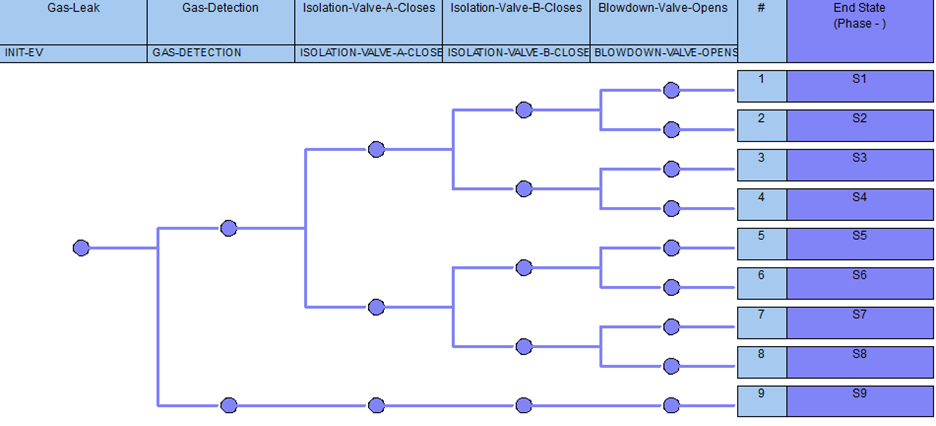
\includegraphics[width=0.9\textwidth]{3_identifying_gaps/benchmarking/datasets/figures/gas_leak_event_tree.png}
    \caption{Gas-leak event tree used in the demonstration model.}
    \label{fig:gas_leak_event_tree}
\end{figure}

Each functional event in the event tree is represented by corresponding fault trees, as shown in Figures~\ref{fig:gas_detection_fault_tree} through \ref{fig:blowdown_valve_fault_tree}.

\begin{figure}[H]
    \centering
    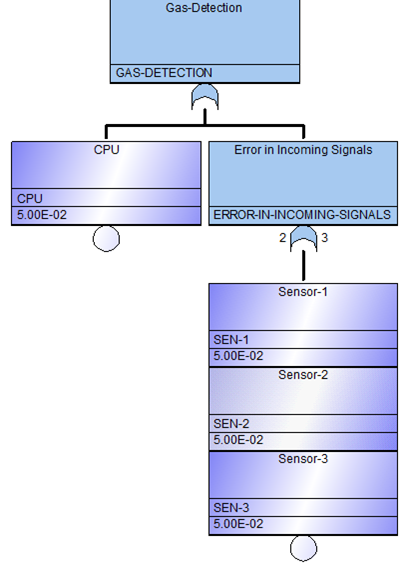
\includegraphics[width=0.4\textwidth]{3_identifying_gaps/benchmarking/datasets/figures/gas_detection_fault_tree.png}
    \caption{Gas-detection system fault tree.}
    \label{fig:gas_detection_fault_tree}
\end{figure}

\begin{figure}[H]
    \centering
    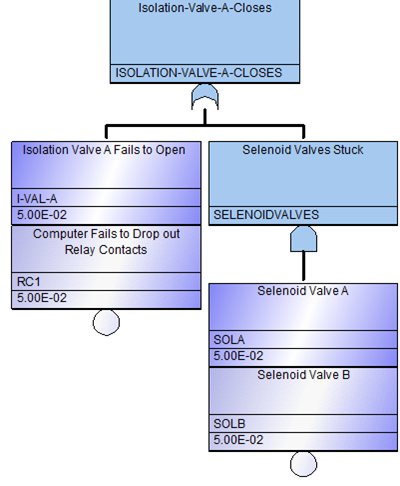
\includegraphics[width=0.4\textwidth]{3_identifying_gaps/benchmarking/datasets/figures/isolation_valve_a_fault_tree.png}
    \caption{Isolation valve A fault tree.}
    \label{fig:isolation_valve_a_fault_tree}
\end{figure}

\begin{figure}[H]
    \centering
    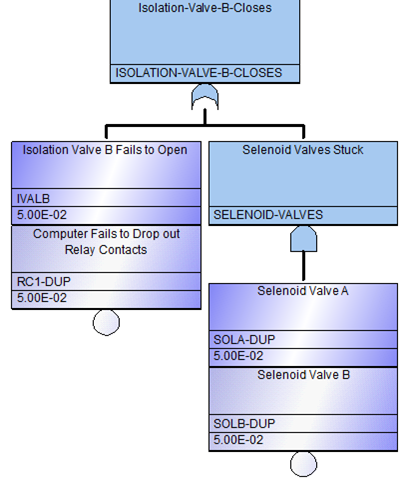
\includegraphics[width=0.4\textwidth]{3_identifying_gaps/benchmarking/datasets/figures/isolation_valve_b_fault_tree.png}
    \caption{Isolation valve B fault tree.}
    \label{fig:isolation_valve_b_fault_tree}
\end{figure}

\begin{figure}[H]
    \centering
    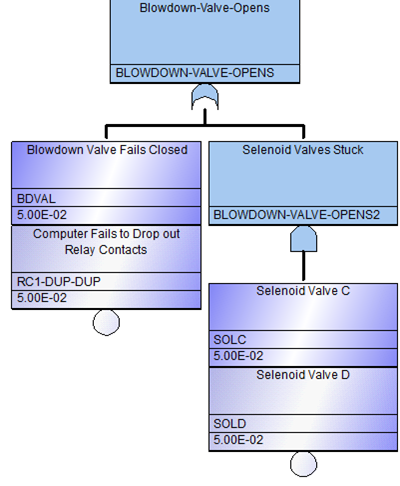
\includegraphics[width=0.4\textwidth]{3_identifying_gaps/benchmarking/datasets/figures/blowdown_valve_fault_tree.png}
    \caption{Blowdown valve fault tree.}
    \label{fig:blowdown_valve_fault_tree}
\end{figure}

The overall model exchange workflow is depicted in Figure~\ref{fig:mef_workflow}. The process is as follows: first, the model is exported from SAPHSOLVE in JSON format. Next, a Python based model converter parses the exported file, mapping its elements to internal objects. The parsed model is then converted to the OpenPSA format, with both JSON and XML representations supported. Finally, the converted model is saved in a text based format suitable for import into other PRA tools.

\begin{figure}[H]
    \centering
    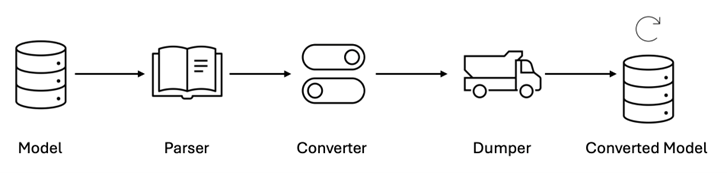
\includegraphics[width=0.7\textwidth]{3_identifying_gaps/benchmarking/datasets/figures/mef_workflow.png}
    \caption{Workflow for engine level model exchange between SAPHIRE and OpenPSA.}
    \label{fig:mef_workflow}
\end{figure}

The mapping of model elements between formats is summarized as follows: the \texttt{header} contains initiating event information, the \texttt{sysgatelist} contains functional event information, the \texttt{sequencelist} contains sequence information, the \texttt{faultreelist} contains fault tree logic, and the \texttt{eventlist} contains basic event failure data. Figure~\ref{fig:mef_demonstration} shows an overview of the mapping process.

\begin{figure}[H]
    \centering
    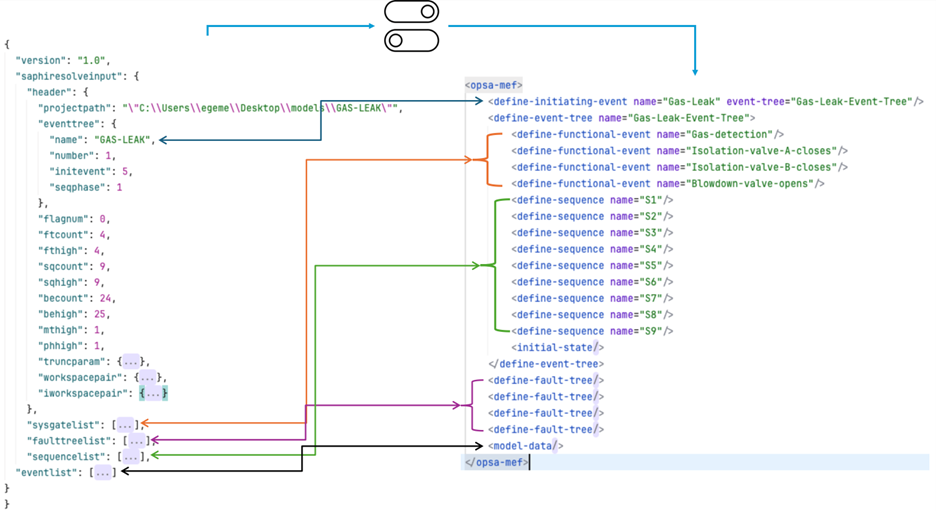
\includegraphics[width=0.9\textwidth]{3_identifying_gaps/benchmarking/datasets/figures/mef_demonstration.png}
    \caption{Demonstration of the mapping and conversion process between SAPHSOLVE and OpenPSA formats.}
    \label{fig:mef_demonstration}
\end{figure}

\subsection{Verification of Model Conversion}

To verify the correctness of the conversion, the resulting OpenPSA model is quantified using the SCRAM engine. The results are compared against those obtained from SAPHSOLVE and the original SCRAM quantification. As shown in Table~\ref{tab:mef_results_comparison}, both the number of cut sets and the computed probabilities are identical across all engines, demonstrating the fidelity of the conversion process.

\begin{table}[htbp]
    \centering
    \caption{Demo model results comparison for SCRAM and SAPHSOLVE.}
    \label{tab:mef_results_comparison}
    \begin{tabular}{|c|c|c|c|c|}
        \hline
        \textbf{Engine Sequence} & \textbf{SCRAM Probability} & \textbf{SCRAM Cut Sets} & \textbf{SAPHIRE Probability} & \textbf{SAPHIRE Cut Sets} \\
        \hline
        S1 & $1.00 \times 10^{0}$ & 1 & $1.00 \times 10^{0}$ & 1 \\
        S2 & $9.98 \times 10^{-2}$ & 3 & $9.98 \times 10^{-2}$ & 3 \\
        S3 & $9.98 \times 10^{-2}$ & 3 & $9.98 \times 10^{-2}$ & 3 \\
        S4 & $1.05 \times 10^{-2}$ & 9 & $1.05 \times 10^{-2}$ & 9 \\
        S5 & $9.98 \times 10^{-2}$ & 3 & $9.98 \times 10^{-2}$ & 3 \\
        S6 & $1.05 \times 10^{-2}$ & 9 & $1.05 \times 10^{-2}$ & 9 \\
        S7 & $1.05 \times 10^{-2}$ & 9 & $1.05 \times 10^{-2}$ & 9 \\
        S8 & $1.08 \times 10^{-3}$ & 27 & $1.08 \times 10^{-3}$ & 27 \\
        S9 & $5.71 \times 10^{-2}$ & 4 & $5.71 \times 10^{-2}$ & 4 \\
        \hline
    \end{tabular}
\end{table}